\section{Sở GD\&ĐT TP. Huế 25--26, Lần 1}

\caulc
\Opensolutionfile{ans}[ans/ans-26-2--SoGD-L1-LC]
\begin{ex}%[Dự án Đề Sở 25-26]%[2D1N1-2]
	Cho hàm số $y=f(x)$ có bảng biến thiên như hình bên dưới.
	\begin{center}
		
\begin{tikzpicture}
			\tkzTabInit[lgt=1.2,espcl=2.5,deltacl=0.5]{$x$ / 0.6, $y'$ / 0.6, $y$ / 2.5}{$-\infty$, $1$, $3$, $+\infty$}
			\tkzTabLine{, +, d, +, 0, -, }
			\tkzTabVar{-/ $-1$, +D-/ $+\infty$ / $-\infty$, +/ $2$, -/ $-\infty$}
		\end{tikzpicture}
	\end{center}
	Hàm số đồng biến trên khoảng nào trong các khoảng dưới đây?
	\choice
	{\True $(2;3)$}
	{$(0;3)$}
	{$(-1;2)$}
	{$(3;4)$}
	\loigiai{
		Dựa vào bảng biến thiên, ta thấy  hàm số đồng biến trên khoảng $(2;3)$.
	}
\end{ex}

\begin{ex}%[Dự án Đề Sở 25-26]%[1H8N2-3]
	\immini{Cho hình chóp $S.ABCD$ có đáy $ABCD$ là hình chữ nhật và $SA \perp (ABCD)$.\\
		Đường thẳng $SA$ \textbf{không} vuông góc với đường thẳng nào trong các đường thẳng sau?
		\choice
		{\True $SC$}
		{$AB$}
		{$AC$}
		{$BD$}}{\begin{tikzpicture}[scale=1,font=\footnotesize,line join = round, line cap = round, >= stealth]
			\coordinate (A) at (0,0);
			\def\x{2}
			\def\y{1.5}
			\def\z{2}
			\def\g{-130}% goc hbh đáy
			\def\n{90} %goc nghiêng
			\coordinate (B) at ($(A)+(\x,0)$);
			\coordinate (C) at ($(B)+(\g:\y)$);
			\coordinate (D) at ($(A)+(C)-(B)$);
			\coordinate (S) at ($(A)+(\n:\z)$);
			\draw (S)--(B)--(C)--cycle;
			\draw (S)--(D)--(C);
			\draw[dashed] (S)--(A)--(B) (D)--(A) (A)--(C) (B)--(D);
			\foreach \p/\g in {A/180,B/-45,C/-45,D/-90,S/90} \draw[fill] (\p) circle(.5pt) node [shift={(\g:.3)}] {$\p$};
	\end{tikzpicture}}
	\loigiai{
		Vì $SA \perp (ABCD)$ nên $SA\perp AC$, suy ra $SA$ không vuông góc với $SC$.
	}
\end{ex}

\begin{ex}%[Dự án Đề Sở 25-26]%[2D1N4-1]
	\immini{Xác định tiệm cận đứng của đồ thị hàm số $y=\dfrac{ax+b}{cx+d}$ có dạng như hình bên.
		\choice
		{$x=1$}
		{\True $x=-1$}
		{$y=1$}
		{$y=-1$}}{\begin{tikzpicture}[scale=.5, font=\footnotesize, line join=round, line cap=round, >=stealth]
			\draw[->] (-5,0)--(0,0) node[below right]{$O$}--(4,0) node[below]{$x$};
			\draw[->] (0,-5) --(0,4) node[right]{$y$};
			
			\draw [domain=-0.6:4, samples=100] %
			plot (\x, {(-1*(\x)+1)/((\x)+1)});
			
			\draw [domain=-5:-1.5, samples=100] %
			plot (\x, {(-1*(\x)+1)/((\x)+1)});
			\draw[fill] (0,0) circle (1pt);
			\foreach \x/\g in {-1/140,1/110} 
			\draw[fill] (\x,0) circle(.5pt)node [shift={(\g:.3)}] {$\x$};
			\foreach \y/\g in {-1/220,1/175} 
			\draw[fill] (0,\y) circle(.5pt)node [shift={(\g:.3)}] {$\y$};
			\draw[blue] (-1,-5)--(-1,4);
			\draw[blue] (-5,-1)--(4,-1);
	\end{tikzpicture}}
	\loigiai{
		Dựa vào đồ thị hàm số, tiệm cận đứng của đồ thị hàm số là $x = -1$.
	}
\end{ex}

\begin{ex}%[Dự án Đề Sở 25-26]%[1D6H4-3]
	Tập nghiệm của bất phương trình $\log_{2}(x-2)>2$ là
	\choice
	{$(4;+\infty)$}
	{$(2;4)$}
	{$(2;+\infty)$}
	{\True $(6;+\infty)$}
	\loigiai{
		Điều kiện $x - 2 > 0 \Leftrightarrow x > 2$.\\
		Ta có $\log_{2}(x-2)>2  \Leftrightarrow x - 2 > 4 \Leftrightarrow x > 6$.\\
		Kết hợp điều kiện, tập nghiệm của bất phương trình là $(6;+\infty)$.
	}
\end{ex}

\begin{ex}%[Dự án Đề Sở 25-26]%[1D2N3-2]
	Cho cấp số nhân $(u_{n})$ biết $u_{3}=4$ và $u_{4}=2$. Tìm công bội $q$ của cấp số nhân đó.
	\choice
	{$q=2$}
	{$q=4$}
	{\True $q=\dfrac{1}{2}$}
	{$q=\sqrt{2}$}
	\loigiai{
		Công bội của cấp số nhân là $q = \dfrac{u_4}{u_3} = \dfrac{2}{4} = \dfrac{1}{2}$.
	}
\end{ex}

\begin{ex}%[Dự án Đề Sở 25-26]%[2D4N1-2]
	Xác định nguyên hàm của hàm số $y=f(x)=2x^{2}$.
	\choice
	{$x^{3}+C$}
	{\True $\dfrac{2x^{3}}{3}+C$}
	{$\dfrac{x^{3}}{3}+C$}
	{$6x^{3}+C$}
	\loigiai{
		Ta có $\displaystyle\int 2x^2\mathrm{\,d}x=\dfrac{2x^3}{3}+C$.
	}
\end{ex}

\begin{ex}%[Dự án Đề Sở 25-26]%[1D1N5-3]
	Xác định tập nghiệm của phương trình $\cos x=1$.
	\choice
	{\True $S=\{k2\pi|k\in\mathbb{Z}\}$}
	{$S=\{\pi+k2\pi|k\in\mathbb{Z}\}$}
	{$S=\{k\pi|k\in\mathbb{Z}\}$}
	{$S=\{\pi+k\pi|k\in\mathbb{Z}\}$}
	\loigiai{
		Ta có $\cos x = 1 \Leftrightarrow x = k2\pi$ với $k \in \mathbb{Z}$.
	}
\end{ex}

\begin{ex}%[Dự án Đề Sở 25-26]%[2H2N2-2]
	Trong không gian với hệ tọa độ $(Oxyz)$, cho điểm $A(2;1;-2)$ và điểm $B(-4;3;4)$. Tọa độ trung điểm $M$ của đoạn $AB$ là
	\choice
	{\True $(-1;2;1)$}
	{$(-2;2;2)$}
	{$(3;2;3)$}
	{$(-2;-2;2)$}
	\loigiai{
		Tọa độ trung điểm $M$ của $AB$ là $M(-1; 2; 1)$.
	}
\end{ex}

\begin{ex}%[Dự án Đề Sở 25-26]%[2H5N1-2]
	Trong không gian $Oxyz$, cho mặt phẳng $(P)$ có phương trình $x-3y+5=0$. Xác định véc-tơ pháp tuyến của mặt phẳng $(P)$.
	\choice
	{\True $\overrightarrow{n}=(1;-3;0)$}
	{$\overrightarrow{n}=(1;0;-3)$}
	{$\overrightarrow{n}=(1;-3;5)$}
	{$\overrightarrow{n}=(1;0;5)$}
	\loigiai{
		Mặt phẳng $(P)\colon 1x - 3y + 0z + 5 = 0$ có một véc-tơ pháp tuyến là $\overrightarrow{n} = (1; -3; 0)$.
	}
\end{ex}

\begin{ex}%[Dự án Đề Sở 25-26]%[0D0N2-2]
	Gieo một con xúc xắc cân đối và đồng chất một lần. Tính xác suất để xúc xắc xuất hiện mặt có số chấm là một số chia hết cho $3$.
	\choice
	{\True $\dfrac{1}{3}$}
	{$\dfrac{1}{2}$}
	{$\dfrac{1}{6}$}
	{$\dfrac{1}{4}$}
	\loigiai{
		Không gian mẫu khi gieo xúc xắc $1$ lần $\Omega = \{1; 2; 3; 4; 5; 6\} \Rightarrow n(\Omega) = 6$.\\
		Gọi $A$ là biến cố \lq\lq xuất hiện mặt có số chấm chia hết cho $3$\rq\rq.\\
		Ta có $A = \{3; 6\} \Rightarrow n(A) = 2$.
		Xác suất $\mathrm{P}(A) = \dfrac{2}{6} = \dfrac{1}{3}$.
	}
\end{ex}

\begin{ex}%[Dự án Đề Sở 25-26]%[2D1N3-]
	\immini{Xác định giá trị nhỏ nhất trên đoạn $[-1;1]$ của hàm số $y=f(x)$ có đồ thị như hình bên.
		\choice
		{$-1$}
		{\True $-4$}
		{$0$}
		{$-2$}}{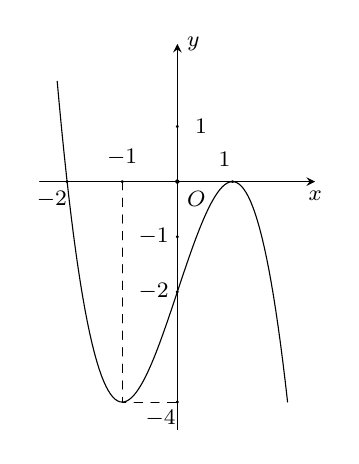
\begin{tikzpicture}[scale=0.7, font=\footnotesize, line join=round, line cap=round, >=stealth]
			\draw[->] (-2.5,0)--(0,0) node[below right]{$O$}--(2.5,0) node[below]{$x$};
			\draw[->] (0,-4.5) --(0,2.5) node[right]{$y$};
			\draw [domain=-2.18:2, samples=100] %
			plot (\x, {-1*(\x+2)*(\x-1)^2});
			\draw[fill] (0,0) circle (1pt);
			\foreach \x/\g in {-2/-130,-1/90,1/110} 
			\draw[fill] (\x,0) circle(.5pt)node [shift={(\g:.3)}] {$\x$};
			\foreach \y/\g in {-4/-135,-2/180,-1/180,1/0} 
			\draw[fill] (0,\y) circle(.5pt)node [shift={(\g:.3)}] {$\y$};
			\draw[dashed] (-1,0)|-(0,-4);
	\end{tikzpicture}}
	\loigiai{
		Dựa vào đồ thị trên đoạn $[-1;1]$, ta thấy giá trị nhỏ nhất của hàm số trên đoạn $[-1;1]$ là $-4$.
	}
\end{ex}

\begin{ex}%[Dự án Đề Sở 25-26]%[2D3N1-2]
	Mỗi ngày bác Bình đều đi bộ để rèn luyện sức khỏe. Quãng đường đi bộ mỗi ngày (đơn vị: km) của bác Bình trong 20 ngày được thống kê ở bảng sau
	\begin{center}
		\begin{tabular}{|l|c|c|c|c|c|}
			\hline
			Quãng đường & $[2;3)$ & $[3;4)$ & $[4;5)$ & $[5;6)$ & $[6;7)$ \\
			\hline
			Số ngày & $3$ & $6$ & $5$ & $4$ & $2$ \\
			\hline
		\end{tabular}
	\end{center}
	Khoảng biến thiên của mẫu số liệu ghép nhóm trên bằng
	\choice
	{$7$}
	{$6$}
	{$1$}
	{\True $5$}
	\loigiai{
		Khoảng biến thiên của mẫu số liệu ghép nhóm là $R = 7 - 2 = 5$.
	}
\end{ex}
\Closesolutionfile{ans}
\cauds
\Opensolutionfile{ans}[ans/ans-26-2--SoGD-L1-DS]
\begin{ex}%[Dự án Đề Sở 25-26]%[2D1H5-4]
	Cho hàm số $y=f(x)=\dfrac{x^{2}-5x+4}{x-5}$ với $x\ne5$.
	\choiceTF
	{\True $f'(x)=1-\dfrac{4}{(x-5)^{2}}$ với mọi $x\neq 5$}
	{\True Đồ thị hàm số cắt trục hoành tại hai điểm phân biệt}
	{\True Hàm số đạt cực đại tại $x=3$}
	{Giá trị cực tiểu bằng $3$}
	\loigiai{
		\begin{itemchoice}
			\itemch Ta có $f(x) = \dfrac{x(x-5) + 4}{x-5} = x + \dfrac{4}{x-5}$ với $x\neq 5$. Suy ra $f'(x) = 1 - \dfrac{4}{(x-5)^2}$ với mọi $x\neq 5$.
			\itemch Phương trình hoành độ giao điểm của đồ thị hàm số và trục $Ox$ là
			$x^2 - 5x + 4 = 0 \Leftrightarrow \hoac{&x=1\\&x=4.}$\\
			Đồ thị cắt trục hoành tại hai điểm phân biệt.
			\itemch Cho $f'(x) = 0 \Leftrightarrow (x-5)^2 = 4 \Leftrightarrow x=7$ hoặc $x=3$.\\
			Bảng xét dấu $y'$
			\begin{center}
				
\begin{tikzpicture}
					\tkzTabInit[lgt=1,espcl=3]
					{$x$/0.7,$y'$/0.7,$y$/2}
					{$-\infty$,$3$,$5$,$7$,$+\infty$}
					\tkzTabLine{,+,$0$,-,d,-,$0$,+,}
					\tkzTabVar{-/$-\infty$,+/1,-D+/$-\infty$/$+\infty$,-/9,+/$+\infty$}
				\end{tikzpicture}
			\end{center}
			Từ bảng xét dấu suy ra hàm số đạt cực đại tại $x=3$.
			\itemch Tại $x=7\Rightarrow y=9$.\\
			Vậy giá trị cực tiểu của hàm số là $9$.
		\end{itemchoice}
	}
\end{ex}

\begin{ex}%[Dự án Đề Sở 25-26]%[2D6V2-4]
	Một hộp có $12$ viên bi gồm $5$ bi xanh, $6$ bi đỏ và $1$ bi vàng. Hai bạn tên là Xanh và Đỏ được trọng tài mời chơi trò chơi bốc bi ngẫu nhiên từ hộp (bi đã lấy ra không bỏ lại vào hộp). Đầu tiên trọng tài bốc một viên bi, nếu là bi xanh hoặc bi đỏ thì dừng bốc, nếu là bi vàng thì trọng tài bốc thêm một viên nữa rồi dừng bốc. Sau khi trọng tài dừng bốc, viên bi trọng tài bốc màu nào thì bạn có tên màu đó sẽ được bốc một viên và ngay sau đó trò chơi dừng lại. Người chơi bốc được viên bi có màu trùng với tên của mình sẽ là người thắng cuộc, còn nếu bốc được viên bi có màu khác với tên của mình sẽ bị thua cuộc.
	\choiceTF
	{\True Xác suất để trọng tài bốc được bi vàng trong lần bốc đầu tiên là $\dfrac{1}{12}$}
	{Giả sử rằng ở lần bốc đầu tiên trọng tài bốc được bi xanh. Khi đó xác suất để bạn Xanh thắng là $\dfrac{5}{11}$}
	{\True Giả sử rằng ở lần bốc đầu tiên trọng tài bốc được bi vàng và bốc tiếp thì được bi đỏ. Khi đó xác suất để bạn Xanh thắng là $\dfrac{1}{2}$}
	{Xác suất để bạn Đỏ thắng là $\dfrac{6}{11}$}
	\loigiai{
		\begin{itemchoice}
			\itemch Số bi vàng là $1$, tổng số bi là $12$. Xác suất bốc bi vàng lần đầu là $\dfrac{1}{12}$.
			\itemch Nếu trọng tài bốc bi xanh, trong hộp còn $11$ viên ($4$ xanh, $6$ đỏ, $1$ vàng). Bạn Xanh được bốc. Để Xanh thắng, Xanh phải bốc được bi xanh. Xác suất này là $\dfrac{4}{11}$.
			\itemch Trọng tài bốc bi vàng, sau đó bốc bi đỏ, trong hộp còn $10$ viên ($5$ xanh, $5$ đỏ). Theo luật, bạn Đỏ sẽ được bốc, bạn Xanh thắng cuộc khi bạn Đỏ bốc được viên bi màu xanh. Xác suất này là $\dfrac{5}{10}=\dfrac{1}{2}$.
			\itemch  Để bạn Đỏ thắng, có các trường hợp sau
			\begin{itemize}  
				\item TH1: Trọng tài bốc bi đỏ lần đầu, sau đó bạn Đỏ bốc được viên bi đỏ.\\ Xác suất này là $\mathrm{P}_1=\dfrac{6}{12}\cdot \dfrac{5}{11}=\dfrac{5}{22}$.\\
				\item TH2: Trọng tài bốc được bi xanh lần đầu, sau đó bạn Xanh bốc được viên không phải màu xanh.\\ Xác suất này là $\mathrm{P}_2=\dfrac{5}{12}\cdot \dfrac{7}{11}=\dfrac{35}{132}$.\\
				\item TH3: Trọng tài bốc được bi vàng lần đầu, lần hai bốc được bi đỏ, sau đó bạn Đỏ bốc được bi đỏ. Xác suất này là $\mathrm{P}_3=\dfrac{1}{12}\cdot\dfrac{6}{11}\cdot\dfrac{5}{10}=\dfrac{1}{44}$.\\
				\item TH4: Trọng tài bốc được bi vàng lần đầu, lần hai bốc được bi xanh, sau đó bạn Xanh bốc được bi đỏ. Xác suất này là $\mathrm{P}_4=\dfrac{1}{12}\cdot\dfrac{5}{11}\cdot\dfrac{6}{10}=\dfrac{1}{44}$.
			\end{itemize}
			Vậy xác suất để bạn Đỏ thắng là $\mathrm{P}_1+\mathrm{P}_2+\mathrm{P}_3+\mathrm{P}_4=\dfrac{5}{22}+\dfrac{35}{132}+\dfrac{1}{44}+\dfrac{1}{44}=\dfrac{71}{132}$.
		\end{itemchoice}
	}
\end{ex}
\begin{ex}%[ Dự án Đề Sở 25-26]%[2D4H3-2]
	\immini
	{Người ta muốn tạo một giá đỡ bằng sắt bên cạnh một bức tường có hình dạng là đoạn cong $BDN$ như hình vẽ bên, giá đỡ được gắn với tường bằng ba thanh sắt $AB$, $CD$, $MN$ cùng vuông góc với tường ($A$, $C$, $M$ thẳng hàng). Giá đỡ được xem như là một phần của đồ thị hàm số $y=\log x$ trong mặt phẳng tọa độ $(Oxy)$ với trục tung trùng với hình chiếu vuông góc của giá đỡ lên mặt tường (đơn vị trên trục tính bằng mét). Biết $A B=10$ cm, $AM=1{,}4$ m và độ dài phần đồ thị của hàm số $y=f(x)$ liên tục trên đoạn $[a;b]$ được tính theo công thức $L=\displaystyle\int\limits_a^b \sqrt{1+\left[f'(x)\right]^2} \mathrm{\,d} x$.}
	{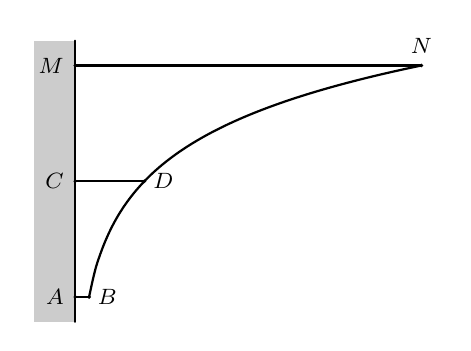
\begin{tikzpicture}[line cap=round,line join=round,>=stealth,font=\footnotesize,x=2.5cm, y=3cm,scale=0.7]
			\def\yA{-1}
			\def\yM{0.4}
			\def\yC{-0.3}
			% Khai báo các tọa độ chính
			\coordinate (A) at (0,\yA);
			\coordinate (B) at ({10^\yA},\yA);
			\coordinate (C) at (0,\yC);
			\coordinate (D) at ({10^\yC},\yC);
			\coordinate (M) at (0,\yM);
			\coordinate (N) at ({10^\yM},\yM);
			% Bức tường (vùng xám)
			\fill[gray!40] (-0.3, \yA - 0.15) rectangle (0, \yM + 0.15);
			\draw[thick] (0, \yA - 0.15) -- (0, \yM + 0.15);
			% Các thanh sắt ngang
			\draw[thick] (A) -- (B);
			\draw[thick] (C) -- (D);
			\draw[thick] (M) -- (N);
			% Đoạn cong BDN (đồ thị hàm số y = log x)
			\draw[thick, smooth, samples=100, domain={10^\yA}:{10^\yM}] plot (\x, {log10(\x)});
			% Vẽ các điểm chấm tròn
			\foreach \p in {A, B, C, D, M, N} {
				\fill (\p) circle (1pt);
			}
			% Gắn nhãn các điểm
			\node[left, inner sep=4pt] at (A) {$A$};
			\node[right, inner sep=3pt] at (B) {$B$};
			\node[left, inner sep=4pt] at (C) {$C$};
			\node[right, inner sep=3pt] at (D) {$D$};
			\node[left, inner sep=4pt] at (M) {$M$};
			\node[above, inner sep=4pt] at (N) {$N$};
	\end{tikzpicture}}
	\choiceTF
	{\True Đạo hàm của hàm số $y=\log x$ là $y'=\dfrac{1}{x \ln 10}$}
	{\True Trong mặt phẳng tọa độ $(Oxy)$, điểm $B$ có hoành độ bằng $0{,}1$}
	{Trong mặt phẳng tọa độ $(Oxy)$, điểm $N$ có tung độ bằng $1{,}4$}
	{\True Độ dài giá đỡ bằng $2{,}97$ mét (\textit{kết quả được làm tròn đến hàng phần trăm})}
	\loigiai{
		\begin{itemchoice}
			\itemch Ta có $y'=\left(\log x\right)'=\dfrac{1}{x\ln 10}$.
			\itemch Ta có $AB=10$ cm $=0{,}1$ m nên $x_B=0{,}1$.
			\itemch Ta có $AM=y_N-y_B\Leftrightarrow 1{,}4=y_N-\log 0{,}1\Leftrightarrow y_N=1{,}4+\log 0{,}1=0{,}4$.
			\itemch Do $y_N=\log x_N$ nên $0{,}4=\log x_N\Leftrightarrow x_N=10^{0{,}4}$. Do vậy, độ dài giá đỡ bằng 
			$$L=\displaystyle\int\limits_{x_B}^{x_N} \sqrt{1+\left[f'(x)\right]^2} \mathrm{\,d} x= \int\limits_{0{,}1}^{10^{0{,}4}}\sqrt{1+\left(\dfrac{1}{x\ln10}\right)^2} \mathrm{\,d} x\approx 2{,}97~\text{(m)}.$$
		\end{itemchoice}
	}
\end{ex}

\begin{ex}%[ Dự án Đề Sở 25-26]%[2H5H2-5]
	Trong không gian với hệ trục tọa độ $(Oxyz)$ cho điểm $A(1;2;3)$ và điểm $B(2;3;4)$. Gọi $M$ là giao điểm của đường thẳng qua hai điểm $A$, $B$ với mặt phẳng $(Oxy)$, $N$ thuộc trục $Oz$ sao cho $AN$ vuông góc với $AB$.
	\choiceTF
	{\True $\overrightarrow{AB}=(1;1;1)$}
	{Hoành độ của điểm $M$ bằng $-1$}
	{$MA=-3AB$}
	{\True $\tan \widehat{NMB}=\dfrac{\sqrt{42}}{9}$}
	\loigiai
	{
		\begin{itemchoice}
			\itemch Ta có $\overrightarrow{AB}=(2-1;3-2;4-3)=(1;1;1)$.
			\itemch Đường thẳng $AB$ đi qua điểm $A(1;2;3)$ và nhận $\overrightarrow{AB}=(2-1;3-2;4-3)=(1;1;1)$ làm vectơ chỉ phương, do đó $$AB\colon \heva{&x=1+t\\&y=2+t\\&z=3+t} (t\in\mathbb{R}).$$
			Mà $M\in AB$ nên $M(1+t;2+t;3+t)$. Mặt khác $M\in (Oxy)$ nên $3+t=0\Leftrightarrow t=-3$.\\
			Do đó $M(-2;-1;0)$ hay $x_M=-2$.
			\itemch Ta có $\overrightarrow{MA}=(3;3;3)$ nên $MA=3\sqrt{3}$. Mặt khác $AB=\sqrt{3}$ nên $MA=3AB$.
			\itemch Do $N\in Oz$ nên $N(0;0;z_N)$. Do đó $\overrightarrow{AN}=(-1;-2;z_N-3)$.\\
			Ta có $AN\perp AB$ nên $\overrightarrow{AN}\cdot\overrightarrow{AB}=0\Leftrightarrow -1-2+z_N-3=0\Leftrightarrow z_N=6$. Suy ra $N(0;0;6)$.\\
			Khi đó $\overrightarrow{MN}=(2;1;6)$ và $\overrightarrow{MB}=(4;4;4)$.\\
			Ta có $\cos \widehat{NMB}=\cos \left(\overrightarrow{MN};\overrightarrow{MB}\right)=\dfrac{\overrightarrow{MN}\cdot \overrightarrow{MB}}{MN\cdot MB}=\dfrac{36}{\sqrt{41}\cdot\sqrt{48}}=\dfrac{3\sqrt{123}}{41}$.\\
			Suy ra $\tan \widehat{NMB}=\dfrac{\sqrt{42}}{9}$.
		\end{itemchoice}
	}
\end{ex}

\Closesolutionfile{ans}


\caukq
\Opensolutionfile{ans}[ans/ans-26-2--SoGD-L1-KQ]
\begin{ex}%[ Dự án Đề Sở 25-26]%[0D0V2-7]
	An và Bình rất giỏi Toán, cùng tham gia một trò chơi, đầu tiên An bốc ngẫu nhiên một thẻ từ hộp thứ nhất chứa sáu thẻ giống nhau được đánh số từ $1$ đến $6$, tiếp theo Bình bốc ngẫu nhiên một thẻ từ hộp thứ hai chứa bốn thẻ giống nhau được đánh số từ $1$ đến $4$. Gọi số An bốc được là $a$ và số của Bình là $b$, sau đó hai người cùng tính giá trị của tích phân $I=\displaystyle\int\limits_0^a x^b \mathrm{\,d}x$. Nếu kết quả $I$ là một số nguyên thì An thắng, ngược lại Bình thắng. Tính xác suất An thắng cuộc (\textit{kết quả làm tròn đến hàng phần trăm}).
	%\shortans{0{,}38}
	\loigiai{
		Do $a\in\{1;2;3;4;5;6\}$ và $b\in\{1;2;3;4\}$ nên $n\left(\Omega\right)=4\cdot 6=24$.\\
		Gọi $A$ là biến cố \lq\lq An thắng cuộc\rq\rq.\\	
		Ta có $I=\displaystyle\int\limits_0^a x^b \mathrm{\,d}x=\dfrac{x^{b+1}}{b+1}\bigg|_0^a=\dfrac{a^{b+1}}{b+1}$. Ta có bốn trường hợp sau
		\begin{itemize}
			\item Trường hợp 1: $b=1$, khi đó $I=\dfrac{a^2}{2}\in\mathbb{Z}\Leftrightarrow a\in\{2;4;6\}$.
			\item Trường hợp 2: $b=2$, khi đó $I=\dfrac{a^3}{3}\in\mathbb{Z}\Leftrightarrow a\in \{3;6\}$.
			\item Trường hợp 3: $b=3$, khi đó $I=\dfrac{a^4}{4}\in\mathbb{Z}\Leftrightarrow a\in \{2;4;6\}$.
			\item Trường hợp 4: $b=4$, khi đó $I=\dfrac{a^5}{5}\in\mathbb{Z}\Leftrightarrow a=5$.
		\end{itemize}
		Do đó $n(A)=3+2+3+1=9$ nên $\mathrm{P}(A)=\dfrac{n(A)}{n(\Omega)}=\dfrac{9}{24}\approx 0{,}38$.
	}
\end{ex}

\begin{ex}%[ Dự án Đề Sở 25-26]%[2H2V1-4]
	\immini{
	Dòng Hương hiền hòa trong xanh, lững lờ trôi giữa lòng thành phố Huế cổ kính và mộng mơ. Nhìn từ trên cao, hai bờ sông trải dài như hai đường thẳng song song. Cột cờ Phu Văn Lâu sừng sững cao $54{,}5$ mét như là một chứng tích hào hùng của lịch sử. Biết rằng hai bờ sông cách nhau $400$ mét và chân cột cờ (hình chiếu vuông góc của đỉnh cột cờ xuống mặt đất) nằm cách mép sông gần nhất một khoảng $200$ mét. Có hai bạn học sinh đứng ở hai bờ sông, bạn học sinh $A$ ở cùng bờ với cột cờ nhìn đỉnh cột cờ so với mặt đất một góc $\alpha$ với tan $\alpha=0{,}1$ và bạn học sinh $B$ đứng ở bờ bên kia nhìn đỉnh cột cờ so với mặt đất một góc $\beta$ với $\tan \beta=0{,}07$. Hỏi hai bạn học sinh cách nhau xa nhất là bao nhiêu mét (\textit{giả sử rằng mặt đất là bằng phẳng và tầm mắt hai bạn học sinh ngang với mặt đất, kết quả làm tròn đến hàng đơn vị})?
	}{
		\begin{tikzpicture}[line cap=round, line join=round, >=stealth, font=\footnotesize,scale=0.6]
			
			\clip (-3.5, -1.5) rectangle (4.5, 5.5);
			\coordinate (H) at (-1.5, 1.5);
			\coordinate (S) at (-1.5, 4.8);
			\coordinate (A) at (3, 1.2);
			\coordinate (B) at (3.5, -0.5);
			\def\bankOneY(#1){0.2*(#1) + 0.6}
			\def\bankTwoY(#1){0.2*(#1) - 1.2}
			\coordinate (L1) at (-4, {\bankOneY(-4)});
			\coordinate (R1) at (5, {\bankOneY(5)});
			\coordinate (L2) at (-4, {\bankTwoY(-4)});
			\coordinate (R2) at (5, {\bankTwoY(5)});
			\path[name path=bank1] (L1) -- (R1);
			\path[name path=HB] (H) -- (B);
			\path [name intersections={of=bank1 and HB, by=I}];
			\fill[cyan!10] (L1) -- (R1) -- (R2) -- (L2) -- cycle;
			\draw[thick, blue!60!black] (L2) -- (R2);
			\draw[thick, blue!60!black] (L1) -- (I);
			\draw[thick, blue!60!black,dashed] (I) -- (A);
			\draw[thick, blue!60!black] (A) -- (R1);
			\draw[thick, blue!70!black] (S) -- (H);
			\draw[thick, blue!70!black] (S) -- (A);
			\draw[thick, blue!70!black] (S) -- (B);
			\draw[thick, dashed, blue!70!black] (H) -- (A);
			\draw[thick, dashed, blue!70!black] (H) -- (B);
			\foreach \p in {S, H, A, B} {
				\fill[red] (\p) circle (1.2pt);
			}
			\node[above, xshift=-0.5mm] at (S) {$S$};
			\node[below left, xshift=1mm, yshift=1mm] at (H) {$H$};
			\node[below left, xshift=1mm] at (A) {$A$};
			\node[below right, xshift=-1mm, yshift=1mm] at (B) {$B$};
			
			\node[left, font=\bfseries\footnotesize, text=black] at ($(S)!0.5!(H)$) {Cột cờ};
			\pic[draw, blue!70!black, angle radius=7mm, "$\alpha$", angle eccentricity=1.3] {angle = S--A--H};
			\pic[draw, blue!70!black, angle radius=7mm, "$\beta$", angle eccentricity=1.3] {angle = S--B--H};
			
		\end{tikzpicture}
	}
	%\shortans{1080}
	\loigiai{
		Ta có $HA=\dfrac{SH}{\tan \alpha}=\dfrac{54{,}5}{0{,}1}=545$ m và $HB=\dfrac{SH}{\tan\beta}=\dfrac{54{,}5}{0{,}07}=778{,}57$ m.\\
		Ta có khoảng cách từ $H$ đến bờ sông chứa bạn $A$ là $d_1=200$ m. Hai bờ sông cách nhau $400$ m nên khoảng cách từ $H$ đến bờ sông chứa bạn $B$ là $d_2=200+400=600$ m.\\
		Ta có khoảng cách dọc theo bờ sông của điểm $A$ so với hình chiếu của $H$ là $$x_A=\sqrt{H A^2-d_1^2}=\sqrt{545^2-200^2} \approx 506{,}98~ \text{(m)}.$$
		Ta có khoảng cách dọc theo bờ sông của điểm $B$ so với hình chiếu của $H$ là 
		$$x_B=\sqrt{H B^2-d_2^2}=\sqrt{\left(\frac{5450}{7}\right)^2-600^2} \approx 496{,}16 ~\text{(m)}.$$
		Ta có để hai bạn cách xa nhau nhất thì $A$ và $B$ phải nằm ở hai phía ngược nhau so với đường vuông góc chung của hai bờ sông kẻ từ $H$. Suy ra bình phương khoảng cách xa nhất là $$A B^2=\left(x_A+x_B\right)^2+400^2=(506{,}98+496{,}16)^2+160\,000 \approx 1\,166\,289.$$
		Vậy khoảng cách lớn nhất $A B=\sqrt{1\,166\,289} \approx 1\,080$ m.
	}
\end{ex}

\begin{ex}%[ Dự án Đề Sở 25-26]%[1D2V3-8]
	Đất sét là một dạng vật chất đặc và mềm, có thể tạo thành nhiều hình dạng khác nhau nhưng thể tích không đổi. Đầu tiên ta có một cục đất sét với thể tích $1\,000$ cm$^3$, người ta nặn thành một khối lập phương đặc, sau đó khoét phần đất sét ở giữa để tạo thành một chậu không nắp (phần trong của chậu có dạng hình hộp chữ nhật) có độ dày bốn mặt bên và độ dày đáy bằng nhau và bằng $\dfrac{1}{10}$ độ dài cạnh của khối lập phương. Phần đất sét còn dư cũng được nặn thành một khối lập phương đặc và cũng khoét phần đất sét ở giữa để tạo thành một chậu không nắp với tỉ lệ giữa độ dày của các mặt và cạnh khối lập phương như trên. Cứ tiếp tục như vậy cho đến khi được $5$ cái chậu. Tính tổng thể tích nước mà $5$ chậu đó có thể chứa (đơn vị là cm$^3$, kết quả làm tròn đến hàng đơn vị).
	%\shortans{1272}
	\loigiai{
		Gọi $V_0 = 1\,000 \text{ cm}^3$ là thể tích của khối lập phương đất sét ban đầu thì cạnh của khối lập phương là $a=10$ cm\\
		Khi khoét phần đất sét ở giữa để tạo thành chậu không nắp, do độ dày các mặt bên và đáy đều bằng $\dfrac{1}{10}a = 0{,}1a$ nên phần không gian chứa nước (lòng chậu) là một hình hộp chữ nhật có
		\begin{itemize}
			\item Đáy là hình vuông với độ dài cạnh là $a - 2 \cdot 0{,}1a = 0{,}8a$.
			\item Chiều cao (do chậu không nắp nên chỉ trừ đi phần đáy) là $a - 0{,}1a = 0{,}9a$.
		\end{itemize}
		Thể tích nước $V_1$ mà chậu này có thể chứa chính là thể tích của phần đất sét bị khoét đi và bằng
		$$V_1 = (0{,}8a)^2 \cdot 0{,}9a = 0{,}576a^3 = 0{,}576V_0.$$
		Gọi $a_1$ là cạnh của khối lập phương thứ hai.\\
		Do chậu tiếp theo cũng được tạo thành theo cách thức như chậu thứ nhất nên thể tích nước $V_2$ mà chậu này có thể chứa chính là thể tích phần đất sét bị khoét đi, và bằng
		$$V_2 = (0{,}8a_1)^2 \cdot 0{,}9a_1 = 0{,}576a_1^3 = 0{,}576V_1.$$
		Tương tự, thể tích nước mà chậu thứ $n$ chứa được sẽ là $V_n = 0{,}576V_{n-1}$.\\
		Như vậy, dãy các thể tích nước mà $5$ chậu chứa được ($V_1, V_2, V_3, V_4, V_5$) tạo thành một cấp số nhân có
		\begin{itemize}
			\item Số hạng đầu: $u_1  = 0{,}576V_0 = 0{,}576 \cdot 1\,000 = 576 \text{ cm}^3$.
			\item Công bội: $q = 0{,}576$.
		\end{itemize}
		Tổng thể tích nước mà $5$ chậu có thể chứa là tổng của $5$ số hạng đầu tiên của cấp số nhân này, nghĩa là
		$$S_5 = u_1 \cdot \dfrac{1 - q^5}{1 - q} = 576 \cdot \dfrac{1 - (0{,}576)^5}{1 - 0{,}576} \approx 1\,272\text{ cm}^3$$
		Làm tròn kết quả đến hàng đơn vị, ta được $1\,272$ cm$^3$.
	}
\end{ex}

\begin{ex}%[ Dự án Đề Sở 25-26]%[0D8V2-7]
	Hằng năm trước ngày Khai giảng năm học mới, Ủy ban nhân dân thành phố Huế giao Sở Giáo dục và Đào tạo tổ chức Lễ Tuyên dương học sinh đạt danh hiệu \lq\lq Học sinh danh dự toàn trường\rq\rq dành cho những học sinh xuất sắc nhất của mỗi trường phổ thông trên địa bàn thành phố. Trong Lễ Tuyên dương, Ban tổ chức vinh danh các học sinh theo lượt nhận, mỗi lượt có $10$ học sinh, với những lượt có $5$ học sinh nam và $5$ học sinh nữ thì Ban tổ chức muốn các học sinh này đứng thành một hàng mà nam nữ xen kẽ. Tuy nhiên khi xếp hàng với lượt có $5$ học sinh nam và $5$ học sinh nữ thì Ban tổ chức nhận thấy các học sinh này không đứng xen kẽ nhưng chỉ cần đổi chỗ hai học sinh nào đó thì được hàng có nam nữ đứng xen kẽ, cách xếp này gọi là \lq\lq cách xếp lỗi\rq\rq. Gọi $D$ là số \lq\lq cách xếp lỗi\rq\rq như trên, xác định giá trị của $\dfrac{D}{100}$.
	%\shortans{$7200$}
	\loigiai{
		Giả sử $10$ vị trí xếp 10 bạn được đánh số từ $1$ đến $10$ như hình sau đây.
		\begin{center}
			\begin{tabular}{|>{\centering}p{1cm}|>{\centering}p{1cm}|>{\centering}p{1cm}|>{\centering}p{1cm}|>{\centering}p{1cm}|>{\centering}p{1cm}|>{\centering}p{1cm}|>{\centering}p{1cm}|>{\centering}p{1cm}|>{\centering\arraybackslash} m{1 cm}|}
				\hline 1 & 2 & 3 & 4 & 5 & 6 & 7 & 8 & 9 & 10 \\ \hline
			\end{tabular}
		\end{center}
		Ta đếm số \lq\lq cách xếp lỗi\rq\rq như sau. \\
		\begin{enumerate}
			\item \textbf{Trường hợp 1:} Có $4$ bạn nam đứng ở vị trí có số lẻ, $1$ bạn nam ở vị trí số chẵn, các bạn nữ vào các vị trí còn lại. 
			\begin{itemize}
				\item Chọn $4$ vị trí mang số lẻ, để xếp $4$ bạn nam có $\mathrm{C}^4_5$ cách (vị trí lẻ còn lại là vị trí của bạn nữ).
				\item Chọn $4$ vị trí mang số chẵn, để xếp $4$ bạn nữ có $\mathrm{C}^4_5$ cách (vị trí chẵn còn lại là vị trí của bạn nam).
				\item Xếp $5$ bạn nam vào các vị trí đã xác định, có $5!$ cách.
				\item Xếp $5$ bạn nữ vào các vị trí đã xác định, có $5!$ cách.
			\end{itemize}
			Vậy trường hợp 1 có $\mathrm{C}^4_5\cdot \mathrm{C}^4_5\cdot 5!\cdot 5!=360\,000$ cách xếp lỗi. 
			\item \textbf{Trường hợp 2:} Có $4$ bạn nữ đứng ở vị trí có số lẻ, $1$ bạn nữ ở vị trí số chẵn, các bạn nam vào các vị trí còn lại. \\
			Tương tự trường hợp $1$, trường hợp $2$ cũng có $360\,000$ cách xếp lỗi.
		\end{enumerate}
		Vậy $\dfrac{D}{100}=\dfrac{360\,000\cdot2}{100}=7\,200$.
	}
\end{ex}

\begin{ex}%[ Dự án Đề Sở 25-26]%[0D3N2-6]
	Một hộ sản xuất và kinh doanh mặt hàng $A$, biết rằng chi phí để sản xuất $x$ kg $(x>0)$ mặt hàng $A$ là $\dfrac{2x^2+x}{x+1}$ (đơn vị triệu đồng), trong lúc đó bán ra mỗi kg là $3$ triệu đồng. Hỏi cần sản xuất bao nhiêu kg mặt hàng $A$ để lợi nhuận đạt $15$ triệu đồng (kết quả làm tròn đến hàng phần chục).
	%\shortans{$14{,}1$}
	\loigiai{
		Lợi nhuận = Doanh thu $-$ Chi phí $= 15$ (triệu đồng).\\
		Doanh thu khi bán $x$ kg là $3x$ triệu đồng.\\
		Chi phí là $\dfrac{2x^2 + x}{x + 1}$ triệu đồng.\\
		Vì lợi nhuận đạt $15$ triệu đồng nên
		{\allowdisplaybreaks
			\begin{eqnarray*}
				3x - \dfrac{2x^2 + x}{x + 1} = 15 &\Leftrightarrow& 3x(x + 1) - (2x^2 + x) = 15(x + 1)\\
				&\Leftrightarrow& x^2 - 13x - 15 = 0\\
				&\Leftrightarrow& x =  \dfrac{13 \pm \sqrt{229}}{2}.
			\end{eqnarray*}
		}
		Vì $x > 0$ nên $x = \dfrac{13 + \sqrt{229}}{2} \approx 14{,}1$.\\
		Cần sản xuất khoảng $14{,}1$ kg mặt hàng $A$.
	}
\end{ex}

\begin{ex}%[ Dự án Đề Sở 25-26]%[1H8V5-4]
	Cho hình chóp cụt tam giác đều $ABC.MNP$ có đáy lớn là tam giác $ABC$ với độ dài cạnh bằng $6$, chiều cao của hình chóp cụt bằng $8$. Gọi $G$ là trọng tâm tam giác $MNP$. Tính khoảng cách giữa hai đường thẳng $AG$ và $BC$ (kết quả làm tròn đến hàng phần trăm).
	%\shortans{$4{,}77$}
	\loigiai{
		\immini{
			Gọi $H$ là trọng tâm $\triangle ABC$. Khi đó $GH$ là chiều cao chóp cụt và $GH=8$.\\
			Gọi $I$ là trung điểm $BC$. Khi đó $BC\perp (AGI)$.\\
			Kẻ $IJ\perp AG$ tại $J$. Khi đó $IJ\perp BC$ (do $BC\perp (AGI)$).\\
			Suy ra $\mathrm{d}(AG,BC)=IJ$. \hfill $(1)$\\
			Kẻ $HK\perp AG$ tại $K$. \\
			Vì $H$ là trọng tâm và theo định lý Thales nên $IJ=\dfrac{3}{2}HK$. \hfill $(2)$\\
			Ta có $AH=\dfrac{2}{3}AI=\dfrac{2}{3}\cdot 6 \cdot \dfrac{\sqrt{3}}{2} = 2\sqrt{3}$.
		}{
			\begin{tikzpicture}[scale=2, line join=round, line cap=round]
				\coordinate[label={left}:{\footnotesize $A$}] (A) at (0,0);       
				\coordinate[label={below}:{\footnotesize $B$}] (B) at (0.8,-0.8);   
				\coordinate[label={right}:{\footnotesize $C$}] (C) at (2.5,0);  
				\coordinate[label={left}:{\footnotesize $M$}] (M) at (0.3, 1.8);        
				\coordinate[label={below left}:{\footnotesize $N$}] (N) at (1, 1.15);      
				\coordinate[label={right}:{\footnotesize $P$}] (P) at (2.05, 1.8);    
				\coordinate (m) at ($(M)!0.5!(P)$);
				\coordinate[label={right}:{\footnotesize $G$}] (G) at ($(N)!0.67!(m)$);
				\coordinate[label={below right}:{\footnotesize $I$}] (I) at ($(B)!0.5!(C)$);
				\coordinate[label={below}:{\footnotesize $H$}] (H) at ($(A)!0.67!(I)$);
				\coordinate[label={above left}:{\footnotesize $J$}] (J) at ($(A)!0.6!(G)$);
				\coordinate[label={above left}:{\footnotesize $K$}] (K) at ($(A)!0.35!(G)$);
				
				\draw[dashed] (C)--(A)--(G)--(H) (A)--(I) (A) (H)--(K) (I)--(J);
				\draw (P)--(N)--(M)--(P)--(C)--(B) (A)--(B)--(N) (M)--(A);
				
				\draw 
				pic[draw, angle radius=2mm]{right angle=G--H--A}
				; 
				\draw 
				pic[draw, angle radius=2mm]{right angle=H--K--A}
				; 
				\draw 
				pic[draw, angle radius=2mm]{right angle=I--J--A}
				; 
				\draw 
				pic[draw, angle radius=2mm]{right angle=A--I--B}
				; 
				
				\foreach \x in {A,B,C,M,N,P,G,N,H,K,I,J} 
				\draw[fill=black] (\x) circle (0.7pt); 
			\end{tikzpicture}
		}
		\noindent Từ đó $HK=\dfrac{HA\cdot HG}{\sqrt{HA^2+HG^2}} = \dfrac{8\sqrt{57}}{19}$. \hfill $(3)$\\
		Từ $(1)$, $(2)$ và $(3)$ suy ra $\mathrm{d}(AG,BC)= \dfrac{3}{2}\cdot \dfrac{8\sqrt{57}}{19} = \dfrac{12\sqrt{3}}{\sqrt{19}} \approx 4{,}77$.
	}
\end{ex}

\Closesolutionfile{ans}

%\indapan{6}{ans/ans-26-2--SoGD-L1-LC}
%\indapan{4}{ans/ans-26-2--SoGD-L1-DS}
%\indapan{6}{ans/ans-26-2--SoGD-L1-KQ}
